\begin{figure}
	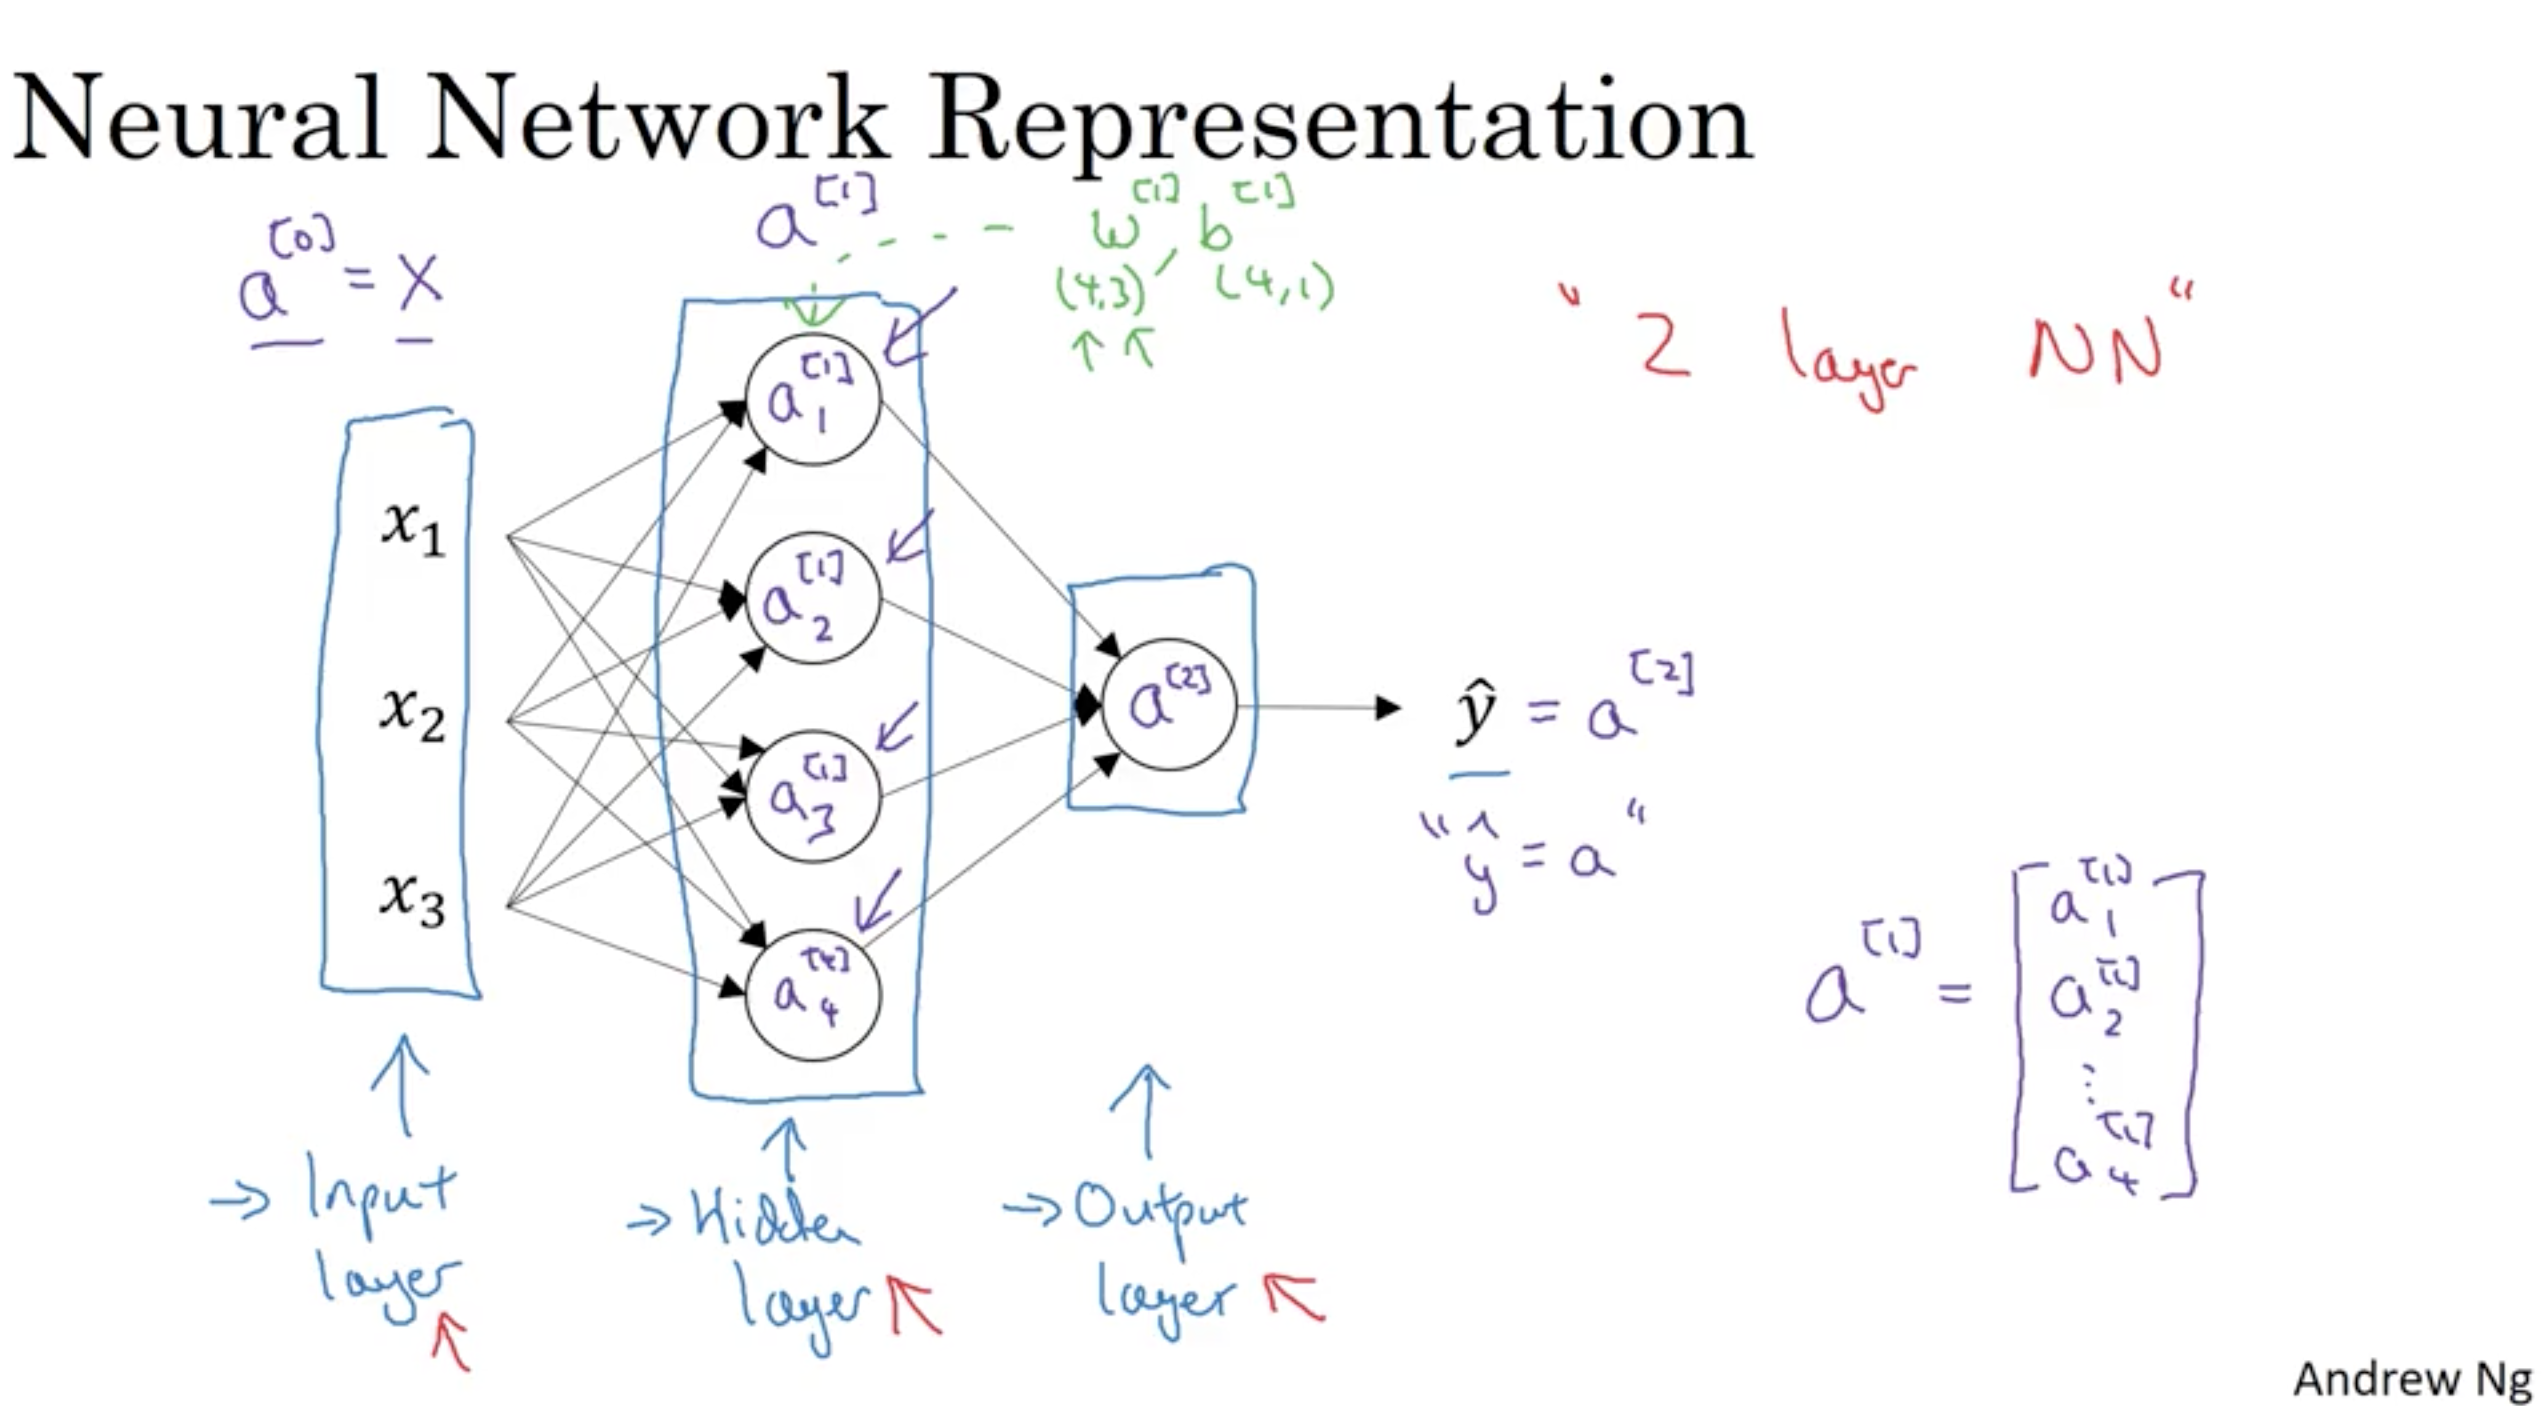
\includegraphics[scale=0.3]{neural_network_representation.png}
	\caption{
		Each node of the neural network corresponds to a different logistic regression computation.
		For example, $a_1^{[1]} = [w_{11}^{[1]}, w_{12}^{[1]}, w_{13}^{[1]}] \times [x_1, x_2, x_3]^T + b_1^{[1]}$.
	}
\end{figure}

$a^{[i](j)}$ is the hidden unit for the $i$-th layer and the $j$-th example.

\subsection{Single example}
	Let $n[i]$ be the number of units in layer $i$.
	In particular, we have $n[0] = n_x$.
	
	\begin{align}
		W^{[i]}\in\mathbb{R}^{n[i]\times n[i-1]}, \quad \forall i\in\{1,\dots,L\} \\
		a^{[i]}, z^{[i]}, b^{[i]} \in \mathbb{R}^{n[i]\times 1} \\
		a^{[0]} = x \\
		z^{[i]} = W^{[i]} a^{[i-1]} + b^{[i]} \\
		a^{[i]} = g^{[i]}(z^{[i]}) \\ 
		\hat{y} = a^{[L]} 
	\end{align}
	
	Where $g^{[i]}(z^{[i]})$ is the activation function of layer $i$.
	There is a total of $L$ hidden layers.
	
	In binary classification, we have $y,\hat{y}\in\{0,1\}$.
	Usually, we use the same cost function as presented for the logistic regression to compute the error
	between the true label $y$ and the prediction $\hat{y}$.

\subsection{Multiple examples}
	\begin{align}
		W^{[i]}\in\mathbb{R}^{n[i]\times n[i-1]}, \quad \forall i\in\{1,\dots,L\} \\
		A^{[i]}, Z^{[i]}, B^{[i]} \in \mathbb{R}^{n[i]\times m} \\
		X \in \mathbb{R}^{n_x \times m} \\
		B^{[i]} = [b^{[i]}, \dots, b^{[i]}]\\
		A^{[0]} = X \\
		Z^{[i]} = W^{[i]} A^{[i-1]} + B^{[i]} \\
		A^{[i]} = g^{[i]}(Z^{[i]}) \\ 
		\hat{Y} = A^{[L]} 
	\end{align}
	
	Since we have multiple examples, we take the mean over all examples for this cost function.
	Let $m$ be the number of examples.
	
	\begin{align}
		Y,\hat{Y}&\in\mathbb{R}^{1\times m} \\
		J(Y, \hat{Y})  &= \frac{1}{m} \sum_{i=1}^{m} \mathcal{L}(Y^{(i)},\hat{Y}^{(i)}) \\
		&= \frac{-1}{m} \sum_{i=1}^{m} \left(
			Y^{(i)} \log(A^{[L](i)}) + (1-Y^{(i)}) \log(1 - A^{[L](i)})
		\right)
	\end{align}

\subsection{Error correction}
	The first forward propagation pass does not produce the best possible results.
	To minimize the cost function $J(Y, \hat{Y})$, we need backward propagation to use the cost of step $i$
	to modify weights of step $i+1$.
	
	Let $E$ be the number of epochs, meaning the number of iterations over all examples of the dataset.
	
	\begin{algorithm}[h]
		Initialize weights $W^{[i]}$ and $b^{[i]}$ for $i\in\{1,\dots,L\}$ \;
		\For{$i=1..E$}{
			Forward propagation to compute $\hat{Y}$\;
			Compute cost $J(Y, \hat{Y})$ \;
			Backpropagation to compute the deltas of weights \;
			Update the weights using $\theta = \theta - \alpha\frac{\delta J}{\delta \theta}$ \;
		}
		\caption{Training algorithm with forward and backward propagation}
	\end{algorithm}

\subsection{Activation functions}
	There are a few possibilities for the activation function of each layer of the neural network.
	Here are the most popular in the litterature.
	
	\begin{center}
	\renewcommand{\arraystretch}{2}
	\begin{tabular}{lll}
		sigmoid & $g(Z^{[l]}) = \frac{1}{1 + \exp^{-Z^{[l]}}}$ 
			& $g'(Z^{[l]}) = g(Z^{[l]}) (1 - g(Z^{[l]}))$\\
		tanh & $g(Z^{[l]}) = \tanh(Z^{[l]}) = \frac{\exp(Z^{[l]}) - \exp(-Z^{[l]})}{\exp(Z^{[l]}) + \exp^{-Z^{[l]}}}$ 
			& $g'(Z^{[l]}) = 1 - (\tanh(Z^{[l]}))^2$\\
		ReLU & $g(Z^{[l]}) = \max(0, Z^{[l]})$ 
			& $g'(Z^{[l]}) = \left\{\begin{array}{cl}
				0 & \mbox{ if } Z^{[l]} < 0 \\
				1 & \mbox{ if } Z^{[l]} \geq 0
			\end{array}\right.$
	\end{tabular}
	\end{center}

\subsection{Regularization}
\begin{align}
	J(Y, \hat{Y})
	&= \frac{1}{m} \sum_{i=1}^{m} \mathcal{L}(Y^{(i)},\hat{Y}^{(i)}) + \frac{\lambda}{2m} \sum_{j=1}^{L} || W^{[j]} ||_F^2 \\
	 || W^{[j]} ||_F^2 &= \sum_{i=1}^{n[j-1]} \sum_{k=1}^{n[j]} (W_{ik})^2 \quad\mbox{(Frobenius norm)} \\
	 dW^{[j]} &= \frac{1}{m}dZ^{[j]} A^{[j-1]} + \frac{\lambda}{m} W^{[j]} \\
	 W^{[j]} &= W^{[j]} - \alpha dW^{[j]} = W^{[j]} - \frac{\alpha}{m} dZ^{[j]} A^{[j-1]} - \frac{\alpha\lambda}{m} W^{[j]} 
\end{align}

\subsection{Parameter initialization}
	Sometimes, we observe exploding or vanishing gradients.
	In order to reduce this effect, we can change the random initialization of the $W$ weights.
	The choice of the random initialization can be an hyperparameter we tune.
	
	The random expressions are written with Python syntax.
	
	\subsubsection{ReLU}
	\[
		W^{[j]} = np.random.randn((n[l],n[l-1])) * \sqrt{\frac{2}{n[l-1]}}
	\]
	
	\subsubsection{tanh}
	\[
		W^{[j]} = np.random.randn((n[l],n[l-1])) * \sqrt{\frac{1}{n[l-1]}}
	\]
	
	\subsubsection{Other}
	The following expression is sometimes also used for the random initialization.
	
	\[
		W^{[j]} = np.random.randn((n[l],n[l-1])) * \sqrt{\frac{2}{n[l-1] + n[l]}}
	\]
	
\subsection{Feature normalization}
	Normalizing features can help with the learning.
	
	Suppose $X\in\mathbb{R}^{n_x\times m}$, where $m$ is the number of examples in the dataset and $n_x$
	is the number of features.
	Let $X^{(i)}_k$ be the $k$-th feature of example $i$.
	
	\begin{align}
		\mu_k				&= \frac{1}{m} \sum_{i=1}^{m} X^{(i)}_k \\
		\sigma^2_k		&= \frac{1}{m} \sum_{i=1}^{m} (X^{(i)}_k)^2 \\
		X^{(i)}_k 			&= \frac{X^{(i)}_k - \mu_k}{\sigma_k^2}, \quad\forall i\in\{1,\dots,m\}
	\end{align}